%
%===================================================================================================
%
\documentclass[11pt,aspectratio=169,professionalfonts]{beamer}
%
%===================================================================================================
%
%
%===================================================================================================
%
% Main Modular Preamble Loader
%
%===================================================================================================

%
%===================================================================================================
%
% Packages
%
%===================================================================================================

\usepackage[absolute,overlay]{textpos}

\usepackage[utf8]{inputenc}
\usepackage[T1]{fontenc}

\usepackage{amsmath}
\usepackage{amsfonts}
\usepackage{amssymb}
% the following order matter!!!
\usepackage{lmodern}
\usepackage{bm}

\usepackage{array}
\usepackage{booktabs}
\usepackage{colortbl}
\usepackage{multirow}

\usepackage{graphicx}
\usepackage{tikz}
\usepackage{pgfplots}

\usepackage{framed}
\usepackage{empheq}

\usepackage{xcolor}
\usepackage{soul}

\usepackage{hyperref}
\usepackage{pgfpages}

%\usepackage{minted}

\usepackage[most]{tcolorbox}
\tcbuselibrary{listings}

\pgfplotsset{compat=1.14}
%
%===================================================================================================
%
% TikZ Libraries
%
%===================================================================================================

\usetikzlibrary{
    arrows.meta,
    positioning,
    fit,
    calc,
    shapes.geometric,
    backgrounds,
    matrix
}

% ── Reusable TikZ styles ─────────────────────────────────────
\tikzset{
  block/.style   = {draw, rounded corners, minimum width=2.0cm,
                    minimum height=0.60cm, align=center, font=\small},
  sblock/.style  = {draw, rounded corners, minimum width=1.4cm,
                    minimum height=0.55cm, align=center, font=\small},
  token/.style   = {draw, rounded corners, minimum width=1.1cm,
                    minimum height=0.55cm, font=\small},
  arr/.style     = {->, thick, boIndigo},
  arrg/.style    = {->, gray!60, line width=0.7pt}
}

%
%===================================================================================================
%
% Custom Colors
%
%===================================================================================================

% General accents
\definecolor{accent}{RGB}{200,60,50}
\definecolor{Accent}{RGB}{240,170,0}
\definecolor{accentblue}{HTML}{457B9D}
\definecolor{accentred}{HTML}{E63946}

% Course colors
\definecolor{CourseBlue}{RGB}{47,53,163}
\definecolor{unibo}{RGB}{0,68,136}
\definecolor{uniboblue}{RGB}{0,54,132}
\definecolor{uniblue}{RGB}{0,76,147}
\definecolor{unired}{RGB}{155,0,20}
\definecolor{codebg}{RGB}{248,248,248}
\definecolor{lightblue}{RGB}{220,235,250}

% Code colors
\definecolor{codebg}{rgb}{0.97,0.97,0.97}
\definecolor{codeborder}{rgb}{0.8,0.8,0.8}

% Neural-network / layer colors
\definecolor{w1col}{RGB}{255,180,0}
\definecolor{w2col}{RGB}{180,90,30}
\definecolor{b1col}{RGB}{0,255,0}
\definecolor{layer1violet}{HTML}{800080}
\definecolor{layer2red}{HTML}{FF0000}
\definecolor{updategreen}{HTML}{228B22}

% Financial colors
\definecolor{finblue}{RGB}{0,51,102}
\definecolor{fingray}{RGB}{100,100,100}
\definecolor{fingreen}{RGB}{0,100,0}
\definecolor{finred}{RGB}{178,34,34}

% Semantic colors
\definecolor{darkgreen}{RGB}{0,120,60}
\definecolor{DeepRed}{RGB}{180,45,45}
\definecolor{Forest}{RGB}{34,120,70}

% Light background colors
\definecolor{lightblue}{RGB}{210,230,250}
\definecolor{lightgreen}{RGB}{210,245,210}
\definecolor{lightorange}{RGB}{255,235,205}
\definecolor{lightred}{RGB}{255,220,220}
\definecolor{lightyellow}{RGB}{255,255,210}

% Soft background colors
\definecolor{SoftBlue}{RGB}{225,235,255}
\definecolor{SoftGray}{RGB}{245,245,245}
\definecolor{SoftGreen}{RGB}{228,243,232}
\definecolor{SoftOrange}{RGB}{255,244,224}

% Modern palette
\definecolor{navy}{RGB}{15,27,61}
\definecolor{deepblue}{RGB}{22,38,83}
\definecolor{midblue}{RGB}{30,58,110}
\definecolor{teal}{RGB}{13,148,136}
\definecolor{lightgray}{RGB}{148,163,184}
\definecolor{ice}{RGB}{202,220,252}
\definecolor{gold}{RGB}{245,158,11}
\definecolor{coral}{RGB}{249,115,22}
\definecolor{darktext}{RGB}{30,41,59}
\definecolor{offwhite}{RGB}{240,244,250}
\definecolor{boIndigo}{RGB}{55,0,153}

\definecolor{NavyBlue}{RGB}{20,40,100}
\definecolor{SteelBlue}{RGB}{70,130,180}
\definecolor{LightGray}{RGB}{245,245,250}
\definecolor{AccentGold}{RGB}{210,160,30}

\definecolor{futC} {gray}{0.60}
\definecolor{actC} {RGB}{15, 82, 186}
\definecolor{doneC}{RGB}{25, 25,  25}

\definecolor{GateOrange}{RGB}{230,120,0}
\definecolor{GatePurple}{RGB}{110,0,150}
\definecolor{CellGold}{RGB}{160,120,0}

% Alias
\colorlet{bolight}{boIndigo!10}
\colorlet{bodark}{boIndigo!85!black}
\colorlet{actFill}{actC!10}   % light-blue cell background when active


%
%===================================================================================================
%
% Beamer Theme and Style
%
%===================================================================================================

\usetheme{Madrid}
\usecolortheme{default}

%
%===================================================================================================
%
% Beamer Color Customization
%
%===================================================================================================

\setbeamercolor{title}{fg=white,bg=CourseBlue}
\setbeamercolor{frametitle}{fg=white,bg=CourseBlue}
\setbeamercolor{structure}{fg=CourseBlue}

\setbeamercolor{block title}{fg=white,bg=CourseBlue}
\setbeamercolor{block body}{fg=black,bg=SoftGray}

\setbeamercolor{item projected}{fg=white,bg=CourseBlue}

\setbeamercolor{section in head/foot}{fg=white,bg=CourseBlue}
\setbeamercolor{subsection in head/foot}{fg=white,bg=CourseBlue!80!black}
\setbeamercolor{author in head/foot}{fg=white,bg=CourseBlue!90!black}
\setbeamercolor{title in head/foot}{fg=white,bg=CourseBlue!70!black}
\setbeamercolor{date in head/foot}{fg=white,bg=CourseBlue!90!black}

%
%===================================================================================================
%
% Navigation Symbols and Itemize Style
%
%===================================================================================================

\setbeamertemplate{navigation symbols}{}

\setbeamertemplate{itemize item}{\color{CourseBlue}$\blacktriangleright$}
\setbeamertemplate{itemize subitem}{\color{CourseBlue}$\bullet$}
%
%===================================================================================================
%
% Mathematical Macros
%
%===================================================================================================

\newcommand{\vect}[1]{\bm{#1}}
\newcommand{\R}{\mathbb{R}}

\newcommand{\bx}{\bm{x}}
\newcommand{\bh}{\bm{h}}
\newcommand{\bw}{\bm{w}}
\newcommand{\bW}{\bm{W}}
\newcommand{\bb}{\bm{b}}
\newcommand{\diag}{\operatorname{diag}}

\newcommand{\vw}{\mathbf{w}}
\newcommand{\vwt}{\tilde{\mathbf{w}}}
%
%===================================================================================================
%
% Text and Highlighting Macros
%
%===================================================================================================

\newcommand{\soft}[1]{\textcolor{CourseBlue}{\textbf{#1}}}

\newcommand{\highlight}[1]{%
    \colorbox{yellow!25}{$\displaystyle #1$}
}

%
%===================================================================================================
%
% Beamer-Compatible Highlight Fix for the soul Package
%
%===================================================================================================

\makeatletter
\let\HL\hl
\renewcommand\hl{%
  \let\set@color\beamerorig@set@color
  \let\reset@color\beamerorig@reset@color
  \HL}
\makeatother

%
%===================================================================================================
%
% Custom Intuition Box
%
%===================================================================================================

\newcommand{\intuition}[1]{%
  \vspace{4pt}
  \begin{tikzpicture}
    \node[
        fill=offwhite,
        rounded corners=4pt,
        inner sep=6pt,
        text width=0.92\textwidth
    ] {%
      \textcolor{teal}{\textbf{Intuition:}} 
      \textcolor{darktext}{\small #1}
    };
  \end{tikzpicture}
}


\newcommand{\dmodel}{d_{\mathrm{model}}}
\newcommand{\dff}{d_{\mathrm{ff}}}
\newcommand{\dk}{d_k}
\newcommand{\dv}{d_v}

% ─────────────────────────────────────────────────────────────────────
%  \drawcell{cx}{cy}{border-color}{fill-color}
%  Draws the RNN cell rectangle + 3 neuron circles at (cx, cy).
% ─────────────────────────────────────────────────────────────────────
\newcommand{\drawcell}[4]{%
  \fill[#4, rounded corners=3pt]
    ({#1-0.68},{#2-1.10}) rectangle ({#1+0.68},{#2+1.10});
  \draw[color=#3, line width=1.5pt, rounded corners=3pt]
    ({#1-0.68},{#2-1.10}) rectangle ({#1+0.68},{#2+1.10});
  \draw[color=#3, line width=0.9pt] (#1,{#2+0.55}) circle(0.21);
  \draw[color=#3, line width=0.9pt] (#1, #2)        circle(0.21);
  \draw[color=#3, line width=0.9pt] (#1,{#2-0.55}) circle(0.21);
}
% Bold vectors shortcut (match existing notation)
\newcommand{\vct}[1]{\bm{#1}}

%
%===================================================================================================
%
\title{Chapter 5 -- Pre-trained Language Models, LLMs and Financial Applications}
\subtitle{Advanced Machine Learning for Finance}
\author{Giovanni Della Lunga}
\institute{University of Bologna}
\date{April-May 2026}
%
%===================================================================================================
%
\AtBeginSection[]{
\begin{frame}
\vfill
\centering
\begin{beamercolorbox}[sep=10pt,center,shadow=true,rounded=true]{title}
\usebeamerfont{title}\insertsectionhead\par
\end{beamercolorbox}
\vfill
\end{frame}
}
%
%===================================================================================================
%
\begin{document}
%
%===================================================================================================
%
\begin{frame}
    \titlepage
\end{frame}
%__________________________________________________________________________
%
\section{Introduction}
%__________________________________________________________________________
%
\begin{frame}{Where We Are in the Course}
  \begin{columns}[T]
    \begin{column}{0.55\linewidth}
      \textbf{Chapter~1 -- Classical NLP}\\
      Bag-of-words, TF-IDF, BM25: sparse,
      high-dimensional, no word-order, no semantics.\\[0.5em]
      \textbf{Chapters~2 \& 3 -- Embeddings and Sequences}\\
      Word2Vec / GloVe: dense but \emph{static}.
      RNNs, LSTMs, encoder-decoder: sequential
      processing, attention seed.\\[0.5em]
      \textbf{Chapter~4 -- Attention and the Transformer}\\
      Scaled dot-product attention, multi-head attention,
      positional encoding, full encoder-decoder stack.
      Encoder-only vs.\ decoder-only split.
    \end{column}
    \begin{column}{0.42\linewidth}
      \begin{block}{Today's question}
        The transformer is the architecture.
        Pre-training sets its parameters.
        Fine-tuning adapts it to a task.
        Retrieval extends its memory.\\[0.4em]
        \emph{When does the result
        add value in a financial workflow --
        and when does it not?}
      \end{block}
    \end{column}
  \end{columns}
\end{frame}
%
%..................................................................
%
\begin{frame}{Why This Chapter Matters}
  \begin{columns}[T]
    \begin{column}{0.48\linewidth}
      \begin{block}{Conceptual reason}
        The pre-training paradigm is the single most
        important shift in applied NLP of the last decade.
        Without understanding it, LLM applications remain
        black boxes and fail in production.
      \end{block}
    \end{column}
    \begin{column}{0.48\linewidth}
      \begin{alertblock}{Practical reason}
        Every financial NLP pipeline built today --
        sentiment classifiers, document extractors,
        RAG question-answering systems -- sits on top
        of one of the models described in this chapter.
      \end{alertblock}
    \end{column}
  \end{columns}
  \vspace{0.6em}
  \begin{exampleblock}{Honest caveat}
    Understanding \emph{how} these models work is also what allows
    you to know \textbf{when not to use them}.
    That is the most important skill in applied machine learning.
  \end{exampleblock}
\end{frame}
%
%..................................................................
%
\begin{frame}{Learning Objectives}
  By the end of this chapter, students should be able to:
  \begin{itemize}
    \item explain the MLM and autoregressive pre-training objectives
          and connect them to the encoder-only / decoder-only split;
    \item describe the fine-tuning paradigm and identify the role of the
          \texttt{[CLS]} token for sentence-level classification;
    \item trace the GPT genealogy and explain why scale produces
          qualitatively new behaviour;
    \item formalise RLHF and explain why alignment carries direct
          financial and legal implications;
    \item construct a RAG pipeline and identify its principal
          failure modes;
    \item apply a \textbf{benchmarking discipline} to financial NLP tasks:
          always measure against the simplest reasonable alternative.
  \end{itemize}
  \vspace{0.3em}
  \begin{alertblock}{Guiding question}
    \emph{Given a trained transformer, how do we use it -- and
    how do we decide whether to use it at all?}
  \end{alertblock}
\end{frame}
%
%..................................................................
%
\begin{frame}{Chapter Roadmap}
  \begin{center}
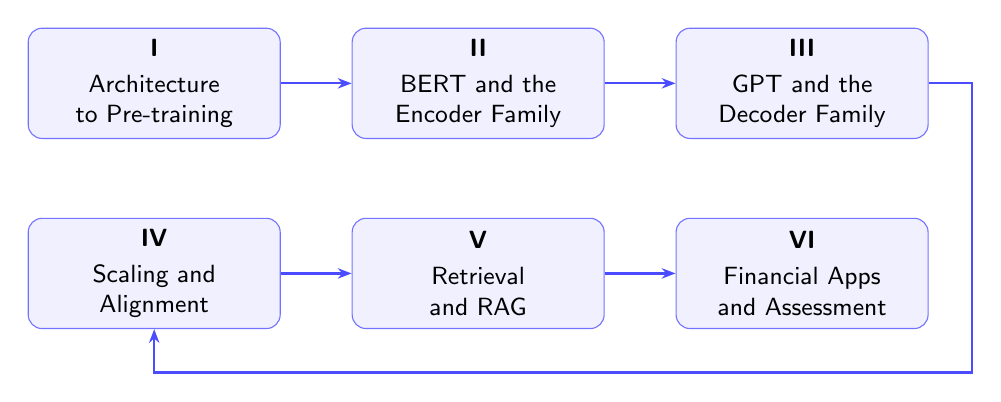
\begin{tikzpicture}[
  node distance=1.0cm and 0.9cm,
  box/.style={
    draw=blue!55,
    fill=blue!6,
    rounded corners=5pt,
    minimum width=3.2cm,
    minimum height=1.4cm,
    align=center,
    font=\sffamily\small
  },
  arr/.style={
    -{Stealth[length=5pt]},
    thick,
    blue!70
  }
]

%% --- Row 1 ---
\node[box] (I) {%
  \textbf{I}\\[2pt]
  Architecture\\to Pre-training};

\node[box, right=of I] (II) {%
  \textbf{II}\\[2pt]
  BERT and the\\Encoder Family};

\node[box, right=of II] (III) {%
  \textbf{III}\\[2pt]
  GPT and the\\Decoder Family};

%% --- Row 2 ---
\node[box, below=of I] (IV) {%
  \textbf{IV}\\[2pt]
  Scaling and\\Alignment};

\node[box, right=of IV] (V) {%
  \textbf{V}\\[2pt]
  Retrieval\\and RAG};

\node[box, right=of V] (VI) {%
  \textbf{VI}\\[2pt]
  Financial Apps\\and Assessment};

%% --- Row 1 arrows ---
\draw[arr] (I)  -- (II);
\draw[arr] (II) -- (III);

%% --- Row 2 arrows (right to left) ---
\draw[arr] (IV) -- (V);
\draw[arr] (V)  -- (VI);

%% --- III -> IV: percorso ESTERNO alla figura ---
%% Va a destra di III, scende sotto tutta la griglia,
%% poi va a sinistra fino a IV.south (senza attraversare la figura).
\draw[arr]
  (III.east)
  -- ++(0.55, 0)                          % esci a destra di III
  |- ($(IV.south) + (0, -0.55)$)          % scendi, poi vai a sinistra sotto IV
  -- (IV.south);                          % risali al bordo inferiore di IV

\end{tikzpicture}
\end{center}
\end{frame}
%__________________________________________________________________________
%
\section{From Architecture to Pre-training}
%__________________________________________________________________________
%
\begin{frame}{The Architecture Is Not the Model}
  Chapter~4 described the transformer as a parametric function:
  \[
    f_{\theta}\,:\;\text{token IDs}\;\longrightarrow\;
    \text{contextual representations}
  \]
  with hundreds of millions of parameters $\theta$.
  \medskip

  \textbf{The architecture specifies only the functional form.}
  The parameters are determined entirely by the training procedure.

  \begin{block}{Two separate questions}
    \begin{itemize}
      \item \textit{Architecture:} how are tokens related inside the forward pass?
            $\;\Rightarrow\;$ answered in Chapters~3 and~4.
      \item \textit{Training:} how are the parameters set?
            $\;\Rightarrow\;$ the subject of this chapter.
    \end{itemize}
  \end{block}
\end{frame}
%
%..................................................................
%
\begin{frame}{Three Paradigms from One Architecture}
  \begin{center}
  \scriptsize
  \renewcommand{\arraystretch}{1.25}
  \begin{tabular}{@{}llll@{}}
    \toprule
    & \textbf{Encoder-only} & \textbf{Decoder-only}
      & \textbf{Encoder-decoder}\\
    \midrule
    Canonical model & BERT & GPT & T5 / BART\\
    Pre-training obj. & Masked LM & Autoregressive LM & Seq2seq denoising\\
    Attention & Bidirectional & Causal masked & Mixed\\
    Token sees & Full context & Past tokens only & Depends on role\\
    Main use & Classify, extract & Generate, prompt & Translate, summarise\\
    \bottomrule
  \end{tabular}
  \end{center}

  \begin{block}{Key insight}
    All three families use the same scaled dot-product attention from Chapter~4.
    The difference is \emph{which positions can attend to which} --
    controlled by the attention mask.
  \end{block}
\end{frame}
%
%..................................................................
%
\begin{frame}{Pre-training as Self-supervised Learning}
  \textbf{Core idea:} train on vast amounts of \emph{raw, unlabelled text}
  by asking the model to predict something about the input itself.
  No human annotation is required -- the labels come from the data.
  \medskip

  \begin{columns}[T]
    \begin{column}{0.48\linewidth}
      \begin{exampleblock}{Encoder: fill the gap (MLM)}
        ``The \texttt{[MASK]} rose sharply after the announcement.''\\
        $\Rightarrow$ predict \emph{yield}.
      \end{exampleblock}
    \end{column}
    \begin{column}{0.48\linewidth}
      \begin{exampleblock}{Decoder: predict next token}
        ``The yield rose sharply after the\ldots''\\
        $\Rightarrow$ predict \emph{announcement}.
      \end{exampleblock}
    \end{column}
  \end{columns}
  \vspace{0.5em}
  \begin{block}{Connection to Chapter~2}
    Word2Vec also learned from self-supervision, but was shallow and task-free.
    Pre-training a deep transformer on billions of tokens produces
    representations that transfer across a wide range of downstream tasks.
  \end{block}
\end{frame}
%
%..................................................................
%
\begin{frame}{Why This Paradigm Changed Everything}
  \begin{columns}[T]
    \begin{column}{0.48\linewidth}
      \textbf{Before pre-training}
      \begin{itemize}
        \item Every task needed a large labelled dataset.
        \item Features were hand-engineered or trained from scratch per task.
        \item Models did not share representations across tasks.
        \item Domain shift required full retraining.
      \end{itemize}
    \end{column}
    \begin{column}{0.48\linewidth}
      \textbf{After pre-training}
      \begin{itemize}
        \item A small labelled dataset is often sufficient.
        \item The model already knows grammar, entities, co-occurrence.
        \item One backbone serves dozens of downstream tasks.
        \item Domain adaptation requires only additional fine-tuning.
      \end{itemize}
    \end{column}
  \end{columns}
  \vspace{0.5em}
  \begin{block}{Illustrative statistic}
    FinBERT (Yang et al.\ 2020) achieves state-of-the-art financial
    sentiment classification using only $\sim$4{,}800 labelled sentences.
    Training a comparable model from scratch would require orders of
    magnitude more labelled data.
  \end{block}
\end{frame}
%__________________________________________________________________________
%
\section{BERT and the Encoder Family}
%__________________________________________________________________________
%
\begin{frame}{Introduction to BERT}
  \textbf{BERT} -- Bidirectional Encoder Representations from Transformers\\
  Devlin, Chang, Lee, Toutanova (Google AI, 2018)
  \medskip

  \begin{itemize}
    \item First model to pre-train a \emph{deep bidirectional} transformer
          using a masked language modelling objective.
    \item Encoder-only: no causal mask -- every token attends to every
          other token in both directions simultaneously.
    \item Achieved new state-of-the-art on 11 NLP benchmarks upon release.
    \item The defining pre-trained model of the 2019--2021 period;
          still the most widely deployed class of models for
          classification and extraction tasks.
  \end{itemize}

  \begin{block}{Central architectural decision}
    Bidirectionality is ideal for \emph{understanding} tasks
    (sentiment, NER, span extraction).
    Its consequence -- inability to generate text autoregressively --
    is a feature, not a bug, for those use cases.
  \end{block}
\end{frame}
%
%..................................................................
%
\begin{frame}{BERT Input Representation}
  For a sequence of tokens $x_1,\ldots,x_n$, the input to BERT is
  the elementwise sum of three embedding vectors:
  \[
    \mathbf{e}_i \;=\;
    \underbrace{\mathbf{e}^{\text{tok}}_i}_{\text{token emb.}}
    +\;
    \underbrace{\mathbf{e}^{\text{seg}}_i}_{\text{segment emb.}}
    +\;
    \underbrace{\mathbf{e}^{\text{pos}}_i}_{\text{position emb.}}
  \]

  \begin{center}
  \small
  \renewcommand{\arraystretch}{1.25}
  \begin{tabular}{@{}ll@{}}
    \toprule
    \textbf{Embedding} & \textbf{What it encodes}\\
    \midrule
    Token & Identity of the WordPiece subword unit\\
    Segment & Sentence A or sentence B (for sentence-pair inputs)\\
    Position & Absolute position in the sequence (\emph{learned}, not sinusoidal)\\
    \bottomrule
  \end{tabular}
  \end{center}
\end{frame}
%
%..................................................................
%
\begin{frame}{BERT Input Representation}
\begin{center}

\includegraphics[scale=.75]{../05-pictures/chapter-05_pic_0.png} 
\end{center}

  \begin{alertblock}{Note on position embeddings}
    Unlike the original transformer (Chapter~4, sinusoidal),
    BERT uses \emph{learned} position embeddings.
    Maximum sequence length is therefore hard-capped at 512 tokens.
  \end{alertblock}

\end{frame}
%
%..................................................................
%
\begin{frame}{WordPiece Tokenization}
  BERT uses \textbf{WordPiece} tokenization: an iterative subword-merging
  algorithm (closely related to BPE from Chapter~1).
  Continuation subwords are prefixed with \texttt{\#\#}:
  \[
    \texttt{playing}\;\to\;\texttt{play}\;+\;\texttt{\#\#ing}
  \]
  \vspace{-.5cm}
  \begin{exampleblock}{Financial examples}
    \renewcommand{\arraystretch}{1.2}
    \begin{tabular}{@{}ll@{}}
      \toprule
      \textbf{Input} & \textbf{WordPiece tokens}\\
      \midrule
      \texttt{non-performing} & \texttt{non}, \texttt{-}, \texttt{performing}\\
      \texttt{EBITDA} & \texttt{EB}, \texttt{\#\#IT}, \texttt{\#\#DA}\\
      \texttt{\$12,345.67} & \texttt{\$}, \texttt{12}, \texttt{,}, \texttt{345}, \texttt{.}, \texttt{67}\\
      \texttt{repo} (repurchase agreement) & \texttt{repo} (single token)\\
      \bottomrule
    \end{tabular}
  \end{exampleblock}
  %\begin{alertblock}{Implication for finance}
  %  Tickers and acronyms may be fragmented into semantically empty pieces.
  %  Domain-specific pre-training builds a vocabulary from financial text,
  %  partially addressing this.
  %\end{alertblock}
\end{frame}
%
%..................................................................
%
\begin{frame}{Special Tokens: \texttt{[CLS]} and \texttt{[SEP]}}
  \begin{columns}[T]
    \begin{column}{0.50\linewidth}
      \textbf{\texttt{[CLS]} -- Classification token}
      \begin{itemize}
        \item Prepended to every input sequence.
        \item No intrinsic meaning at initialisation;
              shaped entirely by training.
        \item After pre-training, its final hidden state
              aggregates sentence-level information.
        \item Used as input to the classification head
              for sentence-level tasks.
      \end{itemize}
    \end{column}
    \begin{column}{0.48\linewidth}
      \textbf{\texttt{[SEP]} -- Separator token}
      \begin{itemize}
        \item Appended at the end of each sentence.
        \item For sentence-pair inputs, separates A from B.
      \end{itemize}
      \vspace{0.5em}
      \textbf{Sentence-pair example:}\\
      {\footnotesize\texttt{[CLS] the yield rose [SEP]\\
      inflation fears drove the move [SEP]}}
    \end{column}
  \end{columns}
  \vspace{0.4em}
  \begin{block}{Key insight}
    The \texttt{[CLS]} output is BERT's understanding \emph{at the
    sentence level}: a single 768-dimensional vector summarising the
    entire input.  For classification, only this vector is fed to the
    downstream head -- all other token representations are discarded.
  \end{block}
\end{frame}
%
%..................................................................
%
\begin{frame}{Pre-training Objective 1: Masked Language Modelling}
\begin{center}

\includegraphics[scale=.65]{../05-pictures/chapter-05_pic_1.png} 
\end{center}
\end{frame}
%
%..................................................................
%
\begin{frame}{Pre-training Objective 1: Masked Language Modelling}

  \textbf{MLM procedure:} select 15\% of input tokens for prediction.
  For each selected token, apply one of three treatments:
  \medskip

  \begin{center}
  \scriptsize
  \renewcommand{\arraystretch}{1.35}

  \begin{tabular}{@{}lll@{}}
    \toprule
    \textbf{Share} & \textbf{Treatment} & \textbf{Example} \\
    \midrule
    \textbf{80\%}
      & Replace with \texttt{[MASK]}
      & ``The yield \texttt{[MASK]} sharply.'' \\

    \textbf{10\%}
      & Replace with a random token
      & ``The yield \emph{river} sharply.'' \\

    \textbf{10\%}
      & Leave unchanged
      & ``The yield \emph{rose} sharply.'' \\
    \bottomrule
  \end{tabular}

  \end{center}

  \medskip

  \textbf{Objective:} predict the original token at each selected position.

  \begin{block}{Why the 80/10/10 split?}
    If only \texttt{[MASK]} were used, pre-training would be too different
    from inference, where no mask tokens appear. The random and unchanged
    cases reduce this mismatch and force the encoder to build useful
    representations for all token positions.
  \end{block}

\end{frame}
%
%..................................................................
%
\begin{frame}{Why MLM Forces Bidirectionality}
  Consider:
  \[
    \text{``The central bank \texttt{[MASK]} interest rates by 50 basis points.''}
  \]
  Predicting the masked word (\emph{raised} / \emph{cut} / \emph{held})
  requires reading \emph{both} left and right context simultaneously.

  \medskip
  \textbf{GPT cannot do this:} the causal mask (Chapter~4) blocks
  right-to-left attention.  Filling a mask with a unidirectional
  model requires a separate bi-directional mechanism.

  \begin{block}{Connection to Chapter~4}
    MLM is the \emph{training signal} that makes bidirectional
    self-attention (no causal mask) maximally useful.
    The masking is applied to the \emph{loss}, not to the attention matrix.
    The encoder attends freely in both directions on every forward pass.
  \end{block}
\end{frame}
%
%..................................................................
%
\begin{frame}{Pre-training Objective 1: Masked Language Modelling}
\begin{center}

\includegraphics[scale=.4]{../05-pictures/chapter-05_pic_2.png} 
\end{center}
\end{frame}
%
%..................................................................
%
\begin{frame}{Pre-training Objective 2: Next Sentence Prediction}
  \textbf{NSP task:} given a token pair
  $[\texttt{CLS}]\;A\;[\texttt{SEP}]\;B\;[\texttt{SEP}]$,
  predict whether $B$ is the actual next sentence following $A$ (IsNext)
  or a randomly sampled sentence (NotNext).

  \begin{itemize}
    \item 50\,\% positive pairs: consecutive sentences from the corpus.
    \item 50\,\% negative pairs: $B$ drawn from a different document.
    \item Prediction made from the \texttt{[CLS]} final hidden state.
  \end{itemize}

  \begin{alertblock}{An honest assessment: NSP is largely useless}
    \textbf{RoBERTa} (Liu et al., 2019) showed that \emph{removing NSP}
    and training on MLM alone with larger batches and more data produces
    a consistently better model on all downstream benchmarks.\\[0.3em]
    Probable reason: random sentence pairs are trivially distinguishable
    without deep inter-sentence reasoning.  The task is too easy.\\[0.3em]
    \textbf{Methodological lesson:} ablation studies matter.
    Intuitive pre-training objectives are not necessarily beneficial.
  \end{alertblock}
\end{frame}
%
%..................................................................
%
\begin{frame}{Pre-training Objective 2: Next Sentence Prediction}
\begin{center}

\includegraphics[scale=.37]{../05-pictures/chapter-05_pic_3.png} 
\end{center}
\end{frame}
%
%..................................................................
%
\begin{frame}{BERT Architecture: Base, Large, and Reference}
  \begin{center}
  \renewcommand{\arraystretch}{1.3}
  \begin{tabular}{@{}lcccc@{}}
    \toprule
    \textbf{Model} & \textbf{Encoder layers}
      & $d_{\text{model}}$ & \textbf{Heads} & \textbf{Parameters}\\
    \midrule
    Transformer (Vaswani 2017) & 6  & 512  &  8 & $\approx$65\,M\\
    BERT-Base                  & 12 & 768  & 12 & 110\,M\\
    BERT-Large                 & 24 & 1024 & 16 & 340\,M\\
    DistilBERT                 &  6 & 768  & 12 &  66\,M\\
    \bottomrule
  \end{tabular}
  \end{center}

  \begin{itemize}
    \item BERT-Base was designed to match the compute of the original
          transformer for fair comparison.
    \item BERT-Large significantly outperforms Base at greater compute cost.
    \item \textbf{DistilBERT} (Sanh et al., 2019): 40\,\% smaller,
          60\,\% faster, retains 97\,\% of BERT-Base performance.
          Preferred for latency-sensitive financial deployments.
  \end{itemize}
\end{frame}
%
%..................................................................
%
\begin{frame}{From Pre-training to Fine-tuning}
  Fine-tuning recipe:
  \begin{enumerate}
    \item \textbf{Initialise} all encoder weights from the pre-trained checkpoint.
    \item \textbf{Add a task-specific head}: a linear layer (or small MLP)
          on top of the \texttt{[CLS]} vector for classification,
          or on top of each token vector for NER and span extraction.
    \item \textbf{Train end-to-end} on the labelled dataset with a
          small learning rate (typically $2$--$5\times10^{-5}$).
  \end{enumerate}

  \begin{columns}[T]
    \begin{column}{0.48\linewidth}
      \begin{block}{Partial freezing}
        Freeze lower encoder layers; update only the top layers and head.
        Faster; useful when the labelled dataset is very small.
      \end{block}
    \end{column}
    \begin{column}{0.48\linewidth}
      \begin{block}{Full fine-tuning}
        Update all parameters.  Achieves best performance when
        sufficient labelled data is available
        ($\gtrsim$1{,}000 examples).
      \end{block}
    \end{column}
  \end{columns}
\end{frame}
%
%..................................................................
%
\begin{frame}{Fine-tuning for Classification: The \texttt{[CLS]} Head}
  For sentence or document classification:
  \[
    \hat{y} \;=\; \mathrm{softmax}\!\bigl(W_c\,\mathbf{h}_{\texttt{[CLS]}}
                                    + \mathbf{b}_c\bigr)
  \]
  where $\mathbf{h}_{\texttt{[CLS]}}\in\mathbb{R}^{d}$ is the final hidden
  state of \texttt{[CLS]} and $W_c\in\mathbb{R}^{K\times d}$ is the
  \emph{only new parameter} to be learned.

  \medskip
  \begin{exampleblock}{Financial example: earnings call sentiment}
    Input: \emph{``Revenue grew 12\,\% year-over-year,
    driven by strong demand in cloud services.''}\\
    Label: positive\\[0.2em]
    This is exactly the task targeted by FinBERT.
    The entire 110\,M-parameter model is fine-tuned on
    $\approx$4{,}800 labelled sentences -- feasible only because of pre-training.
  \end{exampleblock}
\end{frame}
%
%..................................................................
%
\begin{frame}{Fine-tuning for Token-Level Tasks: NER}
  For named entity recognition or extractive question answering,
  \emph{each token position} receives an independent prediction:
  \[
    \hat{y}_i \;=\; \mathrm{softmax}\!\bigl(W_t\,\mathbf{h}_i
                                      + \mathbf{b}_t\bigr),
    \quad i = 1,\ldots,n
  \]
  Same pre-trained backbone; different output head.

  \begin{exampleblock}{Financial NER}
    \begin{itemize}
      \item Extract company names, tickers, dates, and monetary
            figures from SEC filings.
      \item Label risk factors in 10-K documents by type.
      \item Example: ``\underline{Apple} reported revenue of
            \underline{\$117\,B} in \underline{Q4 2023}.''
    \end{itemize}
  \end{exampleblock}
  \begin{block}{Note}
    A single BERT checkpoint can be fine-tuned separately for
    classification (sentence-level head) and NER (token-level head),
    yielding two task-specific models from one pre-trained backbone.
  \end{block}
\end{frame}
%
%..................................................................
%
\begin{frame}{Domain Mismatch Revisited}
  In Chapter~2 we established that general-purpose embeddings
  misrepresent financial terminology.  The same problem afflicts BERT:

  \begin{center}
  \small
  \renewcommand{\arraystretch}{1.25}
  \begin{tabular}{@{}lll@{}}
    \toprule
    \textbf{Term} & \textbf{General nearest neighbour}
      & \textbf{Financial nearest neighbour}\\
    \midrule
    bond  & James Bond, spy, film    & yield, coupon, maturity\\
    call  & phone, ring, dial        & option, strike, put\\
    alpha & Greek, beta, alphabet    & excess return, benchmark\\
    repo  & repository, git, code    & repurchase, overnight, collateral\\
    \bottomrule
  \end{tabular}
  \end{center}

  %\begin{alertblock}{Consequence}
  %  BERT pre-trained on Wikipedia and BookCorpus encodes the
  %  \emph{wrong} neighbourhood structure for financial terms
  %  from the very first layer.
  %  Fine-tuning corrects the head but cannot fully compensate
  %  for the misaligned representations in the lower layers.
  %\end{alertblock}
\end{frame}
%
%..................................................................
%
\begin{frame}{FinBERT: Domain-Specific Pre-training}
  \textbf{FinBERT} (Yang, UY, Huang -- IJCAI 2020):
  continue pre-training BERT-Base on a large financial corpus
  \emph{before} task-specific fine-tuning.

  \begin{itemize}
    \item \textbf{Domain corpus:} Reuters TRC2 financial news,
          Bloomberg financial news, earnings call transcripts.
          $\approx$1.8\,B tokens of financial text.
    \item \textbf{Procedure:} initialise from BERT-Base; continue MLM
          on the financial corpus; fine-tune on the target task.
    \item \textbf{Result on Financial PhraseBank:}
          FinBERT~$\approx$88\,\% vs.\ BERT~$\approx$79\,\% accuracy.
  \end{itemize}

  %\begin{alertblock}{Honest assessment}
  %  The benefit of domain pre-training \emph{shrinks} as the
  %  task-specific labelled dataset grows.
  %  Domain pre-training is most valuable in low-resource settings --
  %  precisely the typical situation in finance.
  %  With 10{,}000+ labelled examples, a well-fine-tuned general BERT
  %  is often competitive with FinBERT.
  %\end{alertblock}
\end{frame}
%
%..................................................................
%
\begin{frame}{BERT: Strengths and Hard Limits}
  \begin{columns}[T]
    \begin{column}{0.48\linewidth}
      \begin{block}{Strengths}
        \begin{itemize}
          \item Strong on classification and extraction
                with small labelled datasets.
          \item Bidirectionality is optimal for understanding.
          \item Fast, auditable, well-understood.
          \item Excellent financial variants on Hugging Face.
          \item DistilBERT for latency-constrained settings.
        \end{itemize}
      \end{block}
    \end{column}
    \begin{column}{0.48\linewidth}
      \begin{alertblock}{Hard limits}
        \begin{itemize}
          %\item \textbf{Cannot generate text.}
          \item \textbf{512-token context:} long financial
                documents (10-K filings) exceed this.
          \item \textbf{Frozen knowledge:} no information
                after the pre-training cutoff.
          \item \textbf{No external memory:} cannot access
                updated information without retraining or RAG.
        \end{itemize}
      \end{alertblock}
    \end{column}
  \end{columns}
\end{frame}
%
%..................................................................
%
\begin{frame}{Encoder Family: Summary}

  \begin{center}
  \scriptsize
  \renewcommand{\arraystretch}{1.3}
  \setlength{\tabcolsep}{3pt}

  \begin{tabular}{@{}llll@{}}
    \toprule
    \textbf{Model}
      & \textbf{Pre-training data}
      & \textbf{Key change}
      & \textbf{Main financial use} \\
    \midrule

    BERT-Base
      & Wikipedia + Books
      & Bidirectional MLM + NSP
      & General baseline \\

    RoBERTa
      & More data
      & No NSP; longer training
      & Stronger baseline \\

    FinBERT
      & Financial corpora
      & Domain adaptation
      & Sentiment; NER \\

    DistilBERT
      & BERT teacher model
      & Smaller and faster
      & Low-latency production \\

    Sentence-BERT
      & NLI / sentence pairs
      & Siamese training
      & Semantic search; RAG \\

    \bottomrule
  \end{tabular}

  \end{center}

\end{frame}%__________________________________________________________________________
%
\section{GPT and the Decoder Family}
%__________________________________________________________________________
%
\begin{frame}{Autoregressive Language Modelling}
  The decoder pre-training objective is classical:
  predict the next token given all previous tokens.
  \[
    \mathcal{L}(\theta)
    \;=\;
    -\sum_{t=1}^{T}
    \log P_\theta\!\bigl(x_t \mid x_1,\ldots,x_{t-1}\bigr)
  \]

  \begin{itemize}
    \item \textbf{No annotation required:} the next token \emph{is} the label.
    \item \textbf{Unbounded self-supervised data:} any text corpus is a
          training set.
    \item \textbf{Causal structure enforced:} position $i$ can only attend
          to positions $1,\ldots,i$ (the causal mask from Chapter~4,
          Section~IV).
  \end{itemize}

  \begin{block}{Distinction from $n$-gram language models}
    Both model the probability of the next token.
    The difference is representational depth: GPT learns rich hierarchical
    contextual representations through transformer self-attention;
    an $n$-gram model counts only fixed-length surface patterns.
  \end{block}
\end{frame}
%
%..................................................................
%
\begin{frame}{Autoregressive Generation: The Expanding Window}
  \textbf{At inference time:}
  \begin{enumerate}
    \item Feed a prompt of $n$ tokens to the model.
    \item Obtain a probability distribution over the full vocabulary:
          $P(x_{n+1}\mid x_1,\ldots,x_n)$.
    \item Sample or select one token $\hat{x}_{n+1}$.
    \item Append $\hat{x}_{n+1}$ to the sequence.
          Go to step~1.
    \item Repeat until a stopping condition is reached
          (end-of-sequence token or maximum length).
  \end{enumerate}

  \begin{alertblock}{Cost structure}
    No single forward pass produces the complete output.
    Each additional token requires one full forward pass over the
    growing sequence.
    Generation cost scales \emph{linearly in output length}.
    For long financial documents, this is a non-trivial infrastructure concern.
  \end{alertblock}
\end{frame}
%
%..................................................................
%
\begin{frame}{Temperature and Top-$p$ Sampling}
  The model outputs a logit vector $\mathbf{z}\in\mathbb{R}^{|V|}$.
  The token probability is:
  \[
    P(x=v\mid\text{context})
    \;=\;
    \frac{\exp(z_v/T)}{\displaystyle\sum_{v'}\exp(z_{v'}/T)}
  \]

  \begin{columns}[T]
    \begin{column}{0.32\linewidth}
      \begin{block}{$T\to 0$: greedy}
        Always pick the argmax.
        Deterministic, focused.
        Use for factual extraction.
      \end{block}
    \end{column}
    \begin{column}{0.32\linewidth}
      \begin{block}{$0{<}T{<}1$: sharp}
        High-prob tokens dominate.
        Low diversity.
      \end{block}
    \end{column}
    \begin{column}{0.32\linewidth}
      \begin{alertblock}{$T{>}1$: flat}
        More randomness.
        \textbf{Never} for outputs that will be acted upon.
      \end{alertblock}
    \end{column}
  \end{columns}
  \vspace{0.5em}
  \textbf{Top-$p$ (nucleus) sampling:} retain the smallest set of tokens
  whose cumulative probability exceeds $p$ (typically 0.90--0.95);
  sample from this nucleus.
  Avoids rare tokens without the rigidity of top-$k$.
\end{frame}
%
%..................................................................
%
\begin{frame}{The GPT Genealogy}
  \begin{center}
  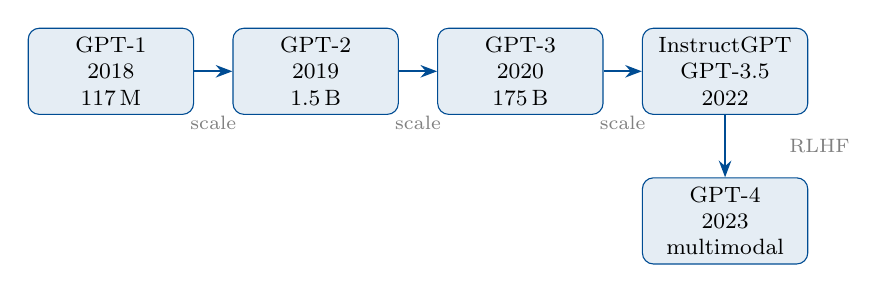
\begin{tikzpicture}[
    nd/.style={draw=uniblue, rounded corners=4pt, fill=uniblue!10,
               minimum width=2.1cm, minimum height=1.0cm,
               align=center, font=\footnotesize},
    arr/.style={-{Stealth[length=6pt]}, thick, uniblue},
    lbl/.style={font=\scriptsize, gray, align=center}
  ]
    \node[nd](g1)  at (0,0)    {GPT-1\\2018\\117\,M};
    \node[nd](g2)  at (2.6,0)  {GPT-2\\2019\\1.5\,B};
    \node[nd](g3)  at (5.2,0)  {GPT-3\\2020\\175\,B};
    \node[nd](g35) at (7.8,0)  {InstructGPT\\GPT-3.5\\2022};
    \node[nd](g4)  at (7.8,-1.9){GPT-4\\2023\\multimodal};
    \draw[arr](g1)--(g2); \draw[arr](g2)--(g3); \draw[arr](g3)--(g35);
    \draw[arr](g35)--(g4);
    \node[lbl] at (1.3,-0.65){scale};
    \node[lbl] at (3.9,-0.65){scale};
    \node[lbl] at (6.5,-0.65){scale};
    \node[lbl] at (9.0,-0.95){RLHF};
  \end{tikzpicture}
  \end{center}
  Three themes across the timeline:
  \begin{itemize}
    \item \textbf{Scale:} parameter count grows by three orders of magnitude.
    \item \textbf{Opacity:} from fully open (GPT-1/2) to closed weights and
          undisclosed training details (GPT-3.5/4).
    \item \textbf{Alignment:} shift from next-token prediction to
          instruction-following via RLHF.
  \end{itemize}
\end{frame}
%
%..................................................................
%
\begin{frame}{GPT-1, GPT-2, and GPT-3}
  \textbf{GPT-1} (Radford et al., 2018 -- 117\,M parameters)\\
  First demonstration: unsupervised pre-training + supervised fine-tuning
  outperforms task-specific architectures trained from scratch.
  \emph{Pre-training learns transferable features.}

  \medskip
  \textbf{GPT-2} (2019 -- 1.5\,B)\\
  Trained on WebText (40\,GB, Reddit outlinks).
  Many tasks can be performed from the prompt alone, with no fine-tuning.
  OpenAI withheld the full model initially -- the first public signal that
  scale creates unexpected capability surprises.

  \medskip
  \textbf{GPT-3} (Brown et al., 2020 -- 175\,B)\\
  The defining discovery: \textbf{in-context learning}.
  \begin{itemize}
    \item \textbf{Zero-shot:} task description in the prompt only.
    \item \textbf{One-shot:} one example input-output pair.
    \item \textbf{Few-shot:} several examples.
  \end{itemize}
  %\begin{alertblock}{Key distinction}
  %  In-context learning involves \textbf{no gradient updates}.
  %  The examples shift the model's implicit prior over the output format;
  %  this is inference, not learning.
  %\end{alertblock}
\end{frame}
%
%..................................................................
%
\begin{frame}{Prompt Engineering and Chain-of-Thought}
  Prompt design has measurable, reproducible effects on output quality.

  \medskip
  \textbf{Chain-of-thought (CoT) prompting} (Wei et al., 2022):\\
  ask the model to reason step by step before giving a final answer.

  \begin{exampleblock}{Financial CoT example}
    \textbf{Prompt:} ``Given the balance sheet data below, determine
    whether the current ratio indicates adequate short-term liquidity.
    Think step by step.''\\[0.2em]
    \textbf{Model:} ``Current assets = \$450\,M.
    Current liabilities = \$380\,M.
    Current ratio $= 450/380 \approx 1.18$.
    A ratio above 1.0 indicates assets exceed liabilities.
    However, 1.18 is thin for a manufacturing company relative to the
    industry median of 1.5\ldots''
  \end{exampleblock}

  \begin{alertblock}{Critical caveat}
    The reasoning chain is fluent and often correct, but can be
    wrong at any step.
    It must be verified against authoritative sources,
    not accepted as a reliable audit trail.
  \end{alertblock}
\end{frame}
%__________________________________________________________________________
%
\section{Scaling Laws and Alignment}
%__________________________________________________________________________
%
\begin{frame}{Scaling Laws}
  \textbf{Kaplan et al.\ (2020):} performance scales as a power law
  in parameters $N$, training tokens $D$, and compute $C$:
  \[
    \mathcal{L}(N) \;\approx\; \Bigl(\frac{N_c}{N}\Bigr)^{\!\alpha_N},
    \qquad
    \mathcal{L}(D) \;\approx\; \Bigl(\frac{D_c}{D}\Bigr)^{\!\alpha_D}
  \]
  Implication: for a fixed compute budget, maximise model size.

  \medskip
  \textbf{Hoffmann et al.\ (2022) -- Chinchilla:}
  the Kaplan law severely \emph{underweights training data}.
  Optimal scaling requires $N$ and $D$ to grow together:
  \[
    N_{\mathrm{opt}} \propto C^{0.5},
    \qquad
    D_{\mathrm{opt}} \propto C^{0.5}
  \]
  \textbf{Chinchilla} (70\,B parameters, 1.4\,T tokens) outperforms
  \textbf{Gopher} (280\,B, 300\,B tokens) on most benchmarks,
  despite having four times fewer parameters.

  \begin{block}{Practical implication}
    Many widely-deployed models are \emph{over-parameterised} relative to
    their training data.  Bigger is not unconditionally better.
  \end{block}
\end{frame}
%
%..................................................................
%
\begin{frame}{Emergent Abilities: What They Are and Why They Are Debated}
  \textbf{Wei et al.\ (2022):} certain abilities (multi-step arithmetic,
  code synthesis) appear to emerge \emph{discontinuously} at threshold scale:
  absent below a parameter count, present above it.

  \medskip
  \textbf{Schaeffer et al.\ (2023):} emergence may be an artefact of
  \emph{non-linear evaluation metrics}.
  With smooth metrics, performance improves continuously.
  The discontinuity is in the metric, not in the model.

  \begin{columns}[T]
    \begin{column}{0.48\linewidth}
      \begin{block}{What practitioners should conclude}
        Emergence is a useful heuristic for capability planning,
        not an established quantitative law.
        Do not assume a capability exists without explicit benchmarking.
      \end{block}
    \end{column}
    \begin{column}{0.48\linewidth}
      \begin{alertblock}{Financial implication}
        A model that appears to understand financial statements on
        standard benchmarks may fail systematically on edge cases
        not present in the evaluation set.
        \textbf{Benchmark on your own data.}
      \end{alertblock}
    \end{column}
  \end{columns}
\end{frame}
%
%..................................................................
%
\begin{frame}{The Alignment Problem and RLHF}
  With GPT-3, the model follows the \emph{statistical structure} of the prompt.
  A model trained on internet text replicates its biases, errors,
  and harmful patterns.

  \textbf{Alignment:} making model behaviour consistent with human
  preferences and values.

  \begin{block}{InstructGPT and RLHF (Ouyang et al., 2022)}
    \textbf{Reinforcement Learning from Human Feedback:}
    train the model to maximise a reward derived from human preferences
    over which of two responses to the same prompt is better.
  \end{block}

  \begin{center}
  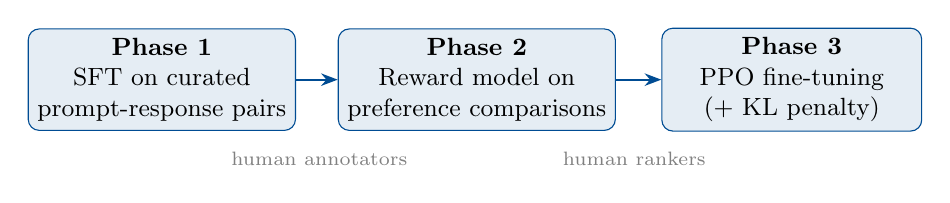
\begin{tikzpicture}[
    box/.style={draw=uniblue, fill=uniblue!10, rounded corners=4pt,
                minimum width=3.3cm, minimum height=1.0cm,
                align=center, font=\small},
    arr/.style={-{Stealth[length=6pt]}, thick, uniblue},
    lbl/.style={font=\scriptsize, gray, align=center}
  ]
    \node[box](sft) at (0,0)   {\textbf{Phase 1}\\SFT on curated\\prompt-response pairs};
    \node[box](rm)  at (4.0,0) {\textbf{Phase 2}\\Reward model on\\preference comparisons};
    \node[box](ppo) at (8.0,0) {\textbf{Phase 3}\\PPO fine-tuning\\(+ KL penalty)};
    \draw[arr](sft)--(rm); \draw[arr](rm)--(ppo);
    \node[lbl] at (2.0,-1){human annotators};
    \node[lbl] at (6.0,-1){human rankers};
  \end{tikzpicture}
  \end{center}

  The \textbf{KL penalty} prevents reward hacking:
  the fine-tuned model is kept close to the SFT baseline.
\end{frame}
%
%..................................................................
%
\begin{frame}{DPO: Direct Preference Optimisation}
  \textbf{Rafailov et al.\ (2023):} RLHF is complex and unstable.
  Training a separate reward model introduces variance;
  PPO is notoriously difficult to tune.

  \medskip
  \textbf{Key insight:} the optimal RLHF policy has a closed form in terms
  of the reference model.  Substituting into the preference likelihood
  yields a \emph{binary cross-entropy loss} on the language model directly:
  \[
    \mathcal{L}_{\mathrm{DPO}}
    \;=\;
    -\mathbb{E}\!\left[\,\log\sigma\!\left(
      \beta\log\frac{\pi_\theta(y_w\mid c)}{\pi_{\mathrm{ref}}(y_w\mid c)}
      \;-\;
      \beta\log\frac{\pi_\theta(y_l\mid c)}{\pi_{\mathrm{ref}}(y_l\mid c)}
    \right)\right]
  \]
  where $y_w$ is the preferred response and $y_l$ the rejected one.

  \begin{block}{Practical consequence}
    DPO requires no reward model and no RL training loop.
    It is now the dominant alignment technique for open-weight models
    due to its simplicity and stability.
  \end{block}
\end{frame}
%
%..................................................................
%
\begin{frame}{Alignment and Finance: A Risk Management Perspective}
  %\begin{alertblock}{Hallucinated financial outputs are not just wrong}
  %  A model that fabricates a credit rating, an earnings figure,
  %  an interest rate, or a regulatory reference does not merely produce
  %  an incorrect output.
  %  In a workflow where model outputs influence decisions,
  %  \textbf{hallucination is a risk management problem},
  %  not an accuracy metric.
  %\end{alertblock}
  %\vspace{0.4em}
  \textbf{Specific scenarios:}
  \begin{itemize}
    \item Model invents a regulatory requirement that does not exist;
          the compliance team acts on it.
    \item Model fabricates a citation to a non-existent research report;
          the analyst includes it in a brief.
    \item Model generates an incorrect numerical summary of a balance sheet;
          the portfolio manager acts on the figure.
  \end{itemize}
  \vspace{0.3em}
  \textbf{Regulatory context:}
  MiFID~II, EU~AI~Act (2024), and US~SR~11-7 create accountability
  requirements for automated outputs that influence investment or
  credit decisions.
  An aligned model reduces risk but is not a substitute for human review.
\end{frame}
%
%..................................................................
%
\begin{frame}{Open Models and the Transparency Imperative}
  \textbf{GPT-4 (2023):} multimodal; improved benchmarks.
  The technical report is 98 pages but discloses almost nothing technical: no architecture, no parameter count, no training data composition.
\vspace{-.3cm}
  \begin{columns}[T]
    \begin{column}{0.48\linewidth}
      \begin{alertblock}{Consequence for finance}
        A black-box commercial model cannot satisfy model risk management,
        audit, or explainability requirements in regulated environments
        (SR~11-7, EU~AI~Act).
        Purchasing from a vendor does not transfer the validation obligation.
      \end{alertblock}
    \end{column}
    \begin{column}{0.48\linewidth}
      \begin{block}{Open alternatives}
        \begin{itemize}
          \item \textbf{LLaMA} (Meta 2023--2024): open weights,
                competitive, deployable on-premises.
          \item \textbf{Mistral-7B:} strong at small scale;
                fits on a single GPU.
          \item \textbf{Gemma, Phi, Falcon:} further options
                with different licence terms.
        \end{itemize}
      \end{block}
    \end{column}
  \end{columns}
  %\vspace{0.3em}
  %\emph{Open weights do not mean full transparency.
  %Evaluate model cards carefully before making auditability claims.}
\end{frame}
%
%..................................................................
%
\begin{frame}{Decoder Family: Summary}

  \begin{center}
  \renewcommand{\arraystretch}{1.3}
  \setlength{\tabcolsep}{3pt}

  \begin{tabular}{@{}llll@{}}
    \toprule
    \textbf{Model}
      & \textbf{Params}
      & \textbf{Key innovation}
      & \textbf{Open weights?} \\
    \midrule

    GPT-2
      & 1.5\,B
      & Zero-shot at scale
      & Yes \\

    GPT-3
      & 175\,B
      & In-context learning
      & No \\

    InstructGPT
      & --
      & RLHF alignment
      & No \\

    GPT-4
      & --
      & Multimodal reasoning
      & No \\

    LLaMA-2
      & 7--70\,B
      & Open-weight LLM family
      & Yes, gated \\

    Mistral-7B
      & 7\,B
      & Strong small model
      & Yes \\

    \bottomrule
  \end{tabular}

  \end{center}

\end{frame}%__________________________________________________________________________
%
\section{Retrieval and RAG}
%__________________________________________________________________________
%
\begin{frame}{The Fundamental Limit: Frozen Knowledge}
  All pre-trained models encode world knowledge in their \textbf{weights}
  at training time.

  \begin{columns}[T]
    \begin{column}{0.48\linewidth}
      \begin{alertblock}{What frozen knowledge means}
        \begin{itemize}
          \item No knowledge of events after the training cutoff.
          \item Cannot access updated earnings, rate decisions,
                or regulatory changes without retraining.
          \item Fine-tuning on new data is expensive, slow,
                and risks catastrophic forgetting.
        \end{itemize}
      \end{alertblock}
    \end{column}
    \begin{column}{0.48\linewidth}
      \begin{block}{The context window as external memory}
        An LLM can read and reason over \emph{any text}
        placed in its context window, even if never seen
        during training.\\[0.4em]
        \textbf{RAG} exploits this: retrieve relevant
        documents at query time, inject them into the prompt,
        generate a grounded answer.
      \end{block}
    \end{column}
  \end{columns}
\end{frame}
%
%..................................................................
%
\begin{frame}{Dense Semantic Search: The Bi-encoder}
  Recall from Chapter~1: BM25 retrieval uses sparse lexical matching.
  Dense retrieval uses \textbf{semantic similarity in embedding space}.

  \medskip
  \textbf{Bi-encoder architecture:}
  \begin{itemize}
    \item Query encoder: $\mathbf{q}=\mathrm{Enc}(q)\in\mathbb{R}^d$
    \item Document encoder: $\mathbf{d}_i=\mathrm{Enc}(d_i)\in\mathbb{R}^d$
    \item Retrieval score:
          $\displaystyle\mathrm{score}(q,d_i)
          =\frac{\mathbf{q}\cdot\mathbf{d}_i}{\|\mathbf{q}\|\,\|\mathbf{d}_i\|}$
  \end{itemize}

  \begin{block}{Key property: offline pre-computation}
    Document vectors are pre-computed and stored.
    Retrieval at query time is a nearest-neighbour search,
    not a full forward pass over each document.
    This makes dense retrieval scalable to millions of documents.
  \end{block}

  %Sentence-BERT (Part~II) is the canonical bi-encoder.
  %Modern alternatives: e5-large, GTE-base, nomic-embed-text.
\end{frame}
%
%..................................................................
%
\begin{frame}{Vector Search at Scale: FAISS}
  Exhaustive cosine search over millions of documents is too slow.

  \textbf{FAISS} (Johnson et al., 2019) provides approximate
  nearest-neighbour search:
  \begin{itemize}
    \item \textbf{Inverted File Index (IVF):} partition the vector space
          into Voronoi cells; at query time, search only the closest cells.
    \item \textbf{Product Quantisation (PQ):} compress vectors into
          short codes, reducing memory and accelerating distance computation.
  \end{itemize}

  \begin{exampleblock}{Practical numbers}
    Millisecond-level retrieval over 10\,M vectors of dimension 768
    on a single GPU.
    IVF + PQ reduces the index for 1\,M documents by 8--32$\times$
    relative to storing full float32 vectors.
  \end{exampleblock}
\end{frame}
%
%..................................................................
%
\begin{frame}{Vector Search at Scale: FAISS}
  \begin{block}{Managed alternatives}
    Qdrant, Weaviate, Pinecone, and similar vector database services
    offer FAISS-style search with additional features (dynamic insertion,
    metadata filtering, hybrid queries).
    Choice depends on update frequency, latency requirements, and
    data residency constraints -- the last being a critical concern for
    financial institutions.
  \end{block}
\end{frame}
%
%..................................................................
%
\begin{frame}{Sparse vs.\ Dense Retrieval Revisited}

  From Chapter~1, sparse and dense methods have
  \textbf{complementary failure modes}:
  \medskip

  \begin{center}
  \renewcommand{\arraystretch}{1.3}
  \setlength{\tabcolsep}{4pt}

  \begin{tabular}{@{}lll@{}}
    \toprule
      & \textbf{Sparse retrieval}
      & \textbf{Dense retrieval} \\
    \midrule

    Method
      & BM25 / lexical matching
      & Bi-encoder embeddings \\

    Strengths
      & Exact terms; names; numbers
      & Synonyms; paraphrases \\

    Failure mode
      & May miss semantic variants
      & May confuse similar meanings \\

    Example
      & Misses ``rate hike''
      & Confuses Apple Inc.\ with fruit \\

    Interpretability
      & High: term scores visible
      & Low: opaque vectors \\

    \bottomrule
  \end{tabular}

  \end{center}
\end{frame}
%
%..................................................................
%
\begin{frame}{Sparse vs.\ Dense Retrieval Revisited}

  \textbf{Hybrid retrieval:} run both methods in parallel and fuse the two
  rankings with \textbf{Reciprocal Rank Fusion (RRF)}:

  \[
    \mathrm{RRF}(d)
    =
    \sum_{r \in \{\mathrm{sparse},\,\mathrm{dense}\}}
    \frac{1}{k + \mathrm{rank}_r(d)}
  \]

  where \(d\) is a document, \(r\) indexes the retrieval method,
  \(\mathrm{rank}_r(d)\) is the rank assigned to document \(d\) by method
  \(r\), and \(k\) is usually set to \(60\).

  \medskip

  No score calibration is required: RRF combines rankings, not raw scores.

\end{frame}
%
%..................................................................
%
\begin{frame}{The RAG Pipeline}
  \begin{center}
  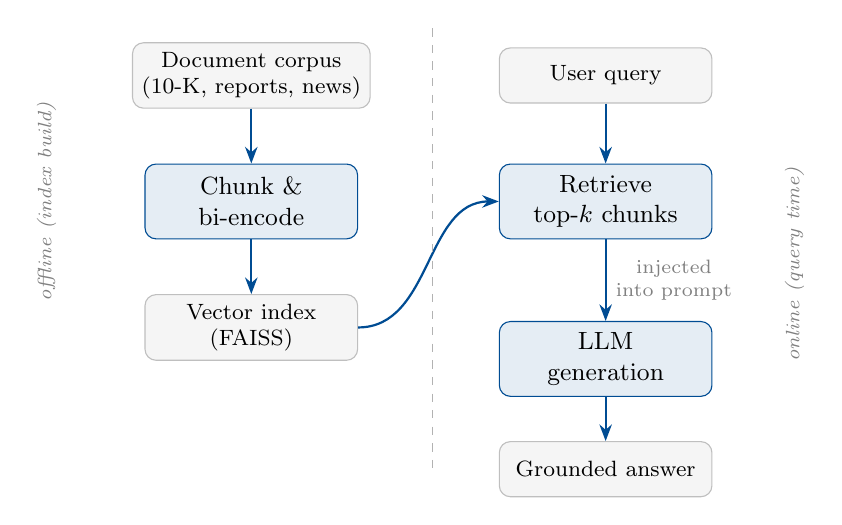
\begin{tikzpicture}[
    box/.style={draw=uniblue, fill=uniblue!10, rounded corners=4pt,
                minimum width=2.7cm, minimum height=0.95cm,
                align=center, font=\small},
    dat/.style={draw=gray!50, fill=gray!8, rounded corners=4pt,
                minimum width=2.7cm, minimum height=0.7cm,
                align=center, font=\footnotesize},
    arr/.style={-{Stealth[length=6pt]}, thick, uniblue},
    lbl/.style={font=\scriptsize, gray, align=center}
  ]
    % Offline
    \node[dat](docs)   at (0, 1.6)  {Document corpus\\(10-K, reports, news)};
    \node[box](chunk)  at (0, 0)    {Chunk \&\\bi-encode};
    \node[dat](idx)    at (0,-1.6)  {Vector index\\(FAISS)};
    % Online
    \node[dat](query)  at (4.5, 1.6){User query};
    \node[box](ret)    at (4.5, 0)  {Retrieve\\top-$k$ chunks};
    \node[box](llm)    at (4.5,-2.0){LLM\\generation};
    \node[dat](ans)    at (4.5,-3.4){Grounded answer};

    \draw[arr](docs)--(chunk); \draw[arr](chunk)--(idx);
    \draw[arr](query)--(ret);
    \draw[arr](idx)  to[out=0,in=180] (ret);
    \draw[arr](ret)  --node[right,lbl]{injected\\into prompt}(llm);
    \draw[arr](llm)--(ans);

    \node[lbl, rotate=90] at (-2.6, 0){\textit{offline (index build)}};
    \node[lbl, rotate=90] at (6.9, -0.8){\textit{online (query time)}};
    \draw[dashed, gray!60](2.3, 2.2)--(2.3,-3.4);
  \end{tikzpicture}
  \end{center}
\end{frame}
%
%..................................................................
%
\begin{frame}{RAG for Financial Text: A Concrete Example}
  \textbf{Task:} ``What are the principal risk factors in this company's
  most recent annual report?''

  \medskip
  \textbf{Offline -- index build:}
  \begin{enumerate}
    \item Chunk the 10-K into 256-token overlapping segments (stride 50).
    \item Encode each chunk with a bi-encoder; store in FAISS.
  \end{enumerate}

  \textbf{Online -- query time:}
  \begin{enumerate}
    \item Encode the query; retrieve top-5 chunks by cosine similarity.
    \item Construct the prompt:
  \end{enumerate}

  \begin{exampleblock}{Prompt structure}
    {\small
    \texttt{System: You are a financial analyst assistant.
    Answer using only the excerpts provided.
    If the information is absent, say so.}\\[0.2em]
    \texttt{[CONTEXT]: \{chunk1\}\ldots\{chunk5\}}\\[0.1em]
    \texttt{[QUESTION]: What are the principal risk factors?}\\[0.1em]
    \texttt{[ANSWER]:}
    }
  \end{exampleblock}
\end{frame}
%
%..................................................................
%
\begin{frame}{Chunking Strategies and Their Trade-offs}

  Chunking is a non-trivial engineering decision with measurable
  effects on retrieval quality.
  \medskip

  \begin{center}
  \scriptsize
  \renewcommand{\arraystretch}{1.3}
  \setlength{\tabcolsep}{4pt}

  \begin{tabular}{@{}lll@{}}
    \toprule
    \textbf{Strategy}
      & \textbf{Advantages}
      & \textbf{Disadvantages} \\
    \midrule

    Fixed-size chunks
      & Simple and uniform
      & May split sentences or tables \\

    Sentence-aware
      & Preserves sentence boundaries
      & Produces uneven lengths \\

    Paragraph-aware
      & Preserves semantic units
      & Long paragraphs may overflow \\

    Overlapping chunks
      & Reduces boundary effects
      & Adds redundancy to the index \\

    \bottomrule
  \end{tabular}

  \end{center}

  \medskip

  \begin{alertblock}{Financial documents require special handling}
    Tables, footnotes, section headers, and numeric exhibits are often
    poorly represented by embeddings trained mainly on prose.
    In production-quality financial RAG systems, structured data usually
    requires a dedicated extraction pipeline.
  \end{alertblock}

\end{frame}
%
%..................................................................
%
\begin{frame}{RAG Failure Modes}
  \begin{enumerate}
    \item \textbf{Retrieval failure.}
          The correct passage is not among the top-$k$ retrieved.
          Regardless of generation quality, the answer will be wrong.\\
          \emph{Measure: recall@$k$ on a held-out question set.}

    \item \textbf{Context poisoning.}
          A retrieved passage is partially relevant and introduces
          misleading context.
          The model generates an answer consistent with the retrieved
          text but incorrect overall.\\
          \emph{Measure: faithfulness -- does the answer follow from
          the retrieved context?}

    \item \textbf{Faithfulness failure.}
          The model ignores the retrieved context and generates a
          plausible answer from its parametric knowledge alone.\\
          \emph{Measure: compare answer against retrieved passages,
          not just against a gold standard.}
  \end{enumerate}

  \begin{block}{Evaluation framework}
    RAGAS (Shahul et al., 2023) provides automated metrics for all three
    failure modes.
    Human evaluation remains necessary for high-stakes financial deployments.
  \end{block}
\end{frame}
%__________________________________________________________________________
%
\section{Hugging Face}
%__________________________________________________________________________
%
\begin{frame}{The Hugging Face Ecosystem}
  Hugging Face provides the standard distribution infrastructure for
  open NLP models:
  \begin{itemize}
    \item \textbf{Model Hub:} $>$500{,}000 models (2025), filterable
          by task, language, licence, and framework.
    \item \textbf{\texttt{transformers} library:} load and run any Hub
          model in a few lines of Python.
    \item \textbf{Model cards:} standardised documentation covering
          training data, evaluation results, intended use, and known
          limitations.
    \item \textbf{Datasets library:} standardised access to NLP
          benchmarks and domain-specific corpora.
  \end{itemize}

  \begin{exampleblock}{Financial models on the Hub (selection)}
    \texttt{ProsusAI/finbert} --
    \texttt{yiyanghkust/finbert-tone} --
    \texttt{nickmuchi/finbert-tone-finetuned-finance-topic-classification}\\
    \texttt{meta-llama/Llama-2-7b-chat-hf} (gated) --
    \texttt{mistralai/Mistral-7B-Instruct-v0.2}
  \end{exampleblock}
\end{frame}
%
%..................................................................
%
\begin{frame}{Model Cards as Due Diligence}
  A model card is not just documentation.
  For a financial institution, it is the \textbf{first step in a model
  risk management process}.

  \medskip
  \textbf{Key fields to inspect before deployment:}
  \begin{itemize}
    \item \textbf{Training data:} composition, time period, known gaps.
    \item \textbf{Evaluation:} which datasets, which metrics, reported numbers.
    \item \textbf{Intended use / out-of-scope use:} does your use case match?
    \item \textbf{Known biases and failure modes:} documented weaknesses.
    \item \textbf{Licence:} can you use it commercially?
          Can you deploy it on-premises?
  \end{itemize}

  \begin{alertblock}{Red flags}
    A model with no card, or a card that omits evaluation details,
    should not be deployed in any production financial workflow without
    independent validation.
    ``Available on Hugging Face'' is not a quality guarantee.
  \end{alertblock}
\end{frame}
%
%..................................................................
%
\begin{frame}[fragile]{A Minimal Working Example}
  \textbf{1.\ Financial sentiment (FinBERT):}
\begin{lstlisting}
from transformers import pipeline
clf = pipeline("text-classification",
               model="ProsusAI/finbert")
clf("Revenue grew 12% driven by strong cloud demand.")
# => [{'label': 'positive', 'score': 0.97}]
\end{lstlisting}
\end{frame}
%
%..................................................................
%
\begin{frame}[fragile]{A Minimal Working Example}
  \textbf{2.\ Sentence similarity (Sentence-BERT):}
\begin{lstlisting}
from sentence_transformers import SentenceTransformer, util
model = SentenceTransformer("all-MiniLM-L6-v2")
embs = model.encode(["yield curve inversion",
                     "inverted yield curve signals recession"])
print(util.cos_sim(embs[0], embs[1]))   # => 0.87
\end{lstlisting}
\end{frame}
%
%..................................................................
%
\begin{frame}[fragile]{A Minimal Working Example}
  \textbf{3.\ Minimal RAG loop (conceptual):}
\begin{lstlisting}
chunks  = retrieve_top_k(query, faiss_index, k=5)
context = "\n".join(chunks)
answer  = llm.generate(
  f"[CONTEXT]: {context}\n[Q]: {query}\n[A]:")
\end{lstlisting}
\end{frame}
%__________________________________________________________________________
%
\section{Financial Applications and Critical Assessment}
%__________________________________________________________________________
%
\begin{frame}{A Taxonomy of Financial NLP Tasks}

  \begin{center}
  \renewcommand{\arraystretch}{1.3}
  \setlength{\tabcolsep}{3pt}

  \begin{tabular}{@{}llll@{}}
    \toprule
    \textbf{Category}
      & \textbf{Financial examples}
      & \textbf{Model family}
      & \textbf{Evidence} \\
    \midrule

    Classification
      & Sentiment; filing category
      & Encoder / FinBERT
      & Strong \\

    Extraction
      & NER; relations; numbers
      & Encoder / token model
      & Strong \\

    Generation
      & Summaries; Q\&A; drafting
      & Decoder + RAG
      & Moderate \\

    Retrieval
      & Semantic search; peer firms
      & Bi-encoder + FAISS
      & Moderate \\

    \bottomrule
  \end{tabular}

  \end{center}

\end{frame}
%
%..................................................................
%
\begin{frame}{The Benchmarking Discipline}
  Before deploying an LLM for any task,
  \textbf{establish a baseline}.

  The baseline is the simplest reasonable alternative:
  \begin{itemize}
    \item Logistic regression on TF-IDF features.
    \item A fine-tuned DistilBERT (66\,M parameters, much faster than BERT-Base).
    \item A rule-based system (dictionary lookup, regex extraction).
  \end{itemize}

  \begin{alertblock}{The discipline in practice}
    \begin{itemize}
      \item An LLM that barely outperforms the baseline is not the right tool.
      \item An LLM that requires $100\times$ more compute to match the
            baseline is \emph{definitely} not the right tool.
      \item A baseline that took one afternoon to build is almost always
            worth building before committing to an LLM pipeline.
    \end{itemize}
  \end{alertblock}

  This connects directly to the course's methodological philosophy:
  method-to-problem fit matters more than method novelty.
\end{frame}
%
%..................................................................
%
\begin{frame}{Known Failure Mode 1: Hallucination}
  \textbf{Hallucination:} the model generates fluent, confident text
  that is factually incorrect.

  \textbf{Financial examples:}
  \begin{itemize}
    \item Fabricated earnings figure: ``the company reported revenue of
          \$12.4\,B in Q3, up 8\,\% year-on-year'' (invented number).
    \item Non-existent regulatory citation.
    \item Incorrect credit rating or index constituent.
  \end{itemize}

  \vspace{0.3em}
  \textbf{Mitigation:}
  \begin{itemize}
    \item RAG with faithfulness evaluation: ground the model in
          retrieved authoritative sources.
    \item Post-hoc numerical verification: extract all numbers from
          the output; cross-reference against a structured database.
    \item Human-in-the-loop for any output that influences a decision.
  \end{itemize}

  \begin{block}{Important}
    Hallucination rate is not zero for any current model on any task.
    It must be \emph{measured}, not assumed away.
  \end{block}
\end{frame}
%
%..................................................................
%
\begin{frame}{Known Failure Mode 2: Temporal Blindness}
  A model trained up to date $T$ has no knowledge of anything after $T$.

  \medskip
  \textbf{In finance, knowledge has a short shelf life:}
  \begin{itemize}
    \item Quarterly earnings, guidance revisions, dividend announcements.
    \item Regulatory updates, ESG reclassifications.
    \item Rate cycle changes, sector rotation.
    \item M\&A events, index reconstitutions.
  \end{itemize}

  \vspace{0.3em}
  \textbf{Mitigation:}
  \begin{itemize}
    \item RAG with a regularly updated and monitored document index.
    \item Report the model's training cutoff date in any output
          that users may act upon.
  \end{itemize}

  \begin{alertblock}{No mitigation is free}
    Regular index updates require pipeline infrastructure and quality
    control.
    They do not eliminate the problem for documents that have not
    yet been indexed.
  \end{alertblock}
\end{frame}
%
%..................................................................
%
\begin{frame}{Known Failure Mode 3: Arithmetic Unreliability}
  LLMs are trained on text.
  Numerical computation was never their objective.

  \medskip
  \textbf{They can fail at:}
  \begin{itemize}
    \item Multi-step arithmetic: $127.3 \times 0.078 - 14.9$.
    \item Percentage change: $\Delta\% = (X_t - X_{t-1})/X_{t-1}$.
    \item Summing a column of figures from a financial table.
    \item Compound interest and present value calculations.
  \end{itemize}

  \vspace{0.3em}
  \textbf{This is not a fixable quirk -- it is architectural.}

  \begin{alertblock}{Design principle}
    Use the LLM for \emph{language understanding}: identify what to compute,
    extract the relevant figures from prose, interpret the result.
    Use \emph{deterministic code} for the arithmetic itself.
    A tool-augmented LLM (function-calling API, Code Interpreter) is the
    correct architecture for tasks that mix natural language and computation.
  \end{alertblock}
\end{frame}
%
%..................................................................
%
\begin{frame}{Known Failure Mode 4: Spurious Confidence}
  RLHF-trained models are incentivised to produce
  \emph{helpful-sounding} responses.
  This can increase overconfidence: the model asserts wrong facts with
  the same tone as correct ones.

  \medskip
  \textbf{Calibration evaluation:}
  \begin{itemize}
    \item \textbf{Expected Calibration Error (ECE):} how well does stated
          confidence track actual accuracy?
    \item \textbf{Selective prediction:} can the model identify which
          outputs are likely wrong?
  \end{itemize}

  \begin{block}{Practical consequence}
    Any LLM output in a financial workflow should be accompanied by
    a confidence estimate and an explicit verification step,
    not a single unqualified assertion.
    A model that says ``I don't know'' is more useful than one that
    says ``The answer is $X$'' when $X$ is wrong.
  \end{block}
\end{frame}
%
%..................................................................
%
\begin{frame}{Regulatory and Governance Considerations}
  \begin{columns}[T]
    \begin{column}{0.48\linewidth}
      \textbf{EU AI Act (2024)}
      \begin{itemize}
        \item LLMs influencing financial decisions likely qualify as
              \emph{high-risk AI systems}.
        \item Requirements: documentation, human oversight, conformity
              assessment, transparency.
        \item General-purpose AI models face additional transparency
              obligations above $10^{25}$ FLOP training compute.
      \end{itemize}
    \end{column}
    \begin{column}{0.48\linewidth}
      \textbf{Model Risk Management (SR~11-7 / SS1/23)}
      \begin{itemize}
        \item US~Fed / UK~PRA guidelines require validation,
              ongoing monitoring, and documentation for all models
              influencing decisions.
        \item Scope includes statistical algorithms, ML models,
              and by extension LLM components.
        \item Purchasing from a vendor does not transfer the
              validation obligation.
      \end{itemize}
    \end{column}
  \end{columns}
\end{frame}
%
%..................................................................
%
\begin{frame}{Regulatory and Governance Considerations}
  \vspace{0.4em}
  \begin{alertblock}{Key message}
    Regulatory compliance requires model transparency, validation,
    and audit trails.
    A model card is a starting point,
    not a substitute for internal model risk management.
  \end{alertblock}
\end{frame}
%
%..................................................................
%
\begin{frame}{What the Evidence Shows}
  \begin{columns}[T]
    \begin{column}{0.48\linewidth}
      \begin{block}{Documented production successes}
        \begin{itemize}
          \item Financial sentiment classification at scale.
          \item Named entity recognition in SEC filings.
          \item Earnings call summarisation and search.
          \item Compliance document classification.
          \item Internal chatbots for regulatory Q\&A.
        \end{itemize}
      \end{block}
    \end{column}
    \begin{column}{0.48\linewidth}
      \begin{alertblock}{Claims that exceed evidence}
        \begin{itemize}
          \item Autonomous alpha generation from LLM text signals.
          \item Macro-economic forecasting from news summaries.
          \item Reliable credit risk assessment from unstructured text.
          \item Financial reasoning without programmatic verification.
        \end{itemize}
      \end{alertblock}
    \end{column}
  \end{columns}
  %\vspace{0.5em}
  %\begin{exampleblock}{The pattern to watch for}
  %  \textbf{Hype displacement:} replacing a working system with an LLM
  %  because it is new, not because it demonstrably improves on
  %  a well-measured baseline.
  %  The benchmarking discipline is the defence against this.
  % \end{exampleblock}
\end{frame}
%__________________________________________________________________________
%
\section{Conclusion and References}
%__________________________________________________________________________
%
\begin{frame}{Chapter~5 -- Key Takeaways}
  \begin{enumerate}
    \item The \textbf{pre-training / fine-tuning paradigm} decouples
          language knowledge (from scale, no labels) from task adaptation
          (small labelled datasets).
    \item \textbf{BERT} uses MLM to train a deep bidirectional encoder;
          the \texttt{[CLS]} representation enables classification
          with a minimal task-specific head.
    \item \textbf{Domain mismatch} is real: financial terminology requires
          domain-specific pre-training (FinBERT) or fine-tuning on
          domain-labelled data.
    \item \textbf{GPT / autoregressive models} generate text token by token;
          temperature and top-$p$ control stochasticity.
    \item \textbf{RLHF / DPO} make models follow instructions;
          alignment is a financial risk management concern, not only ethical.
    \item \textbf{RAG} extends LLM memory via retrieval; it mitigates but
          does not eliminate hallucination, temporal blindness, or
          faithfulness failures.
    \item The \textbf{benchmarking discipline}: always measure against the
          simplest reasonable alternative before committing to an LLM solution.
  \end{enumerate}
\end{frame}
%
%..................................................................
%
\begin{frame}{The Full Course Arc}
  \begin{center}
  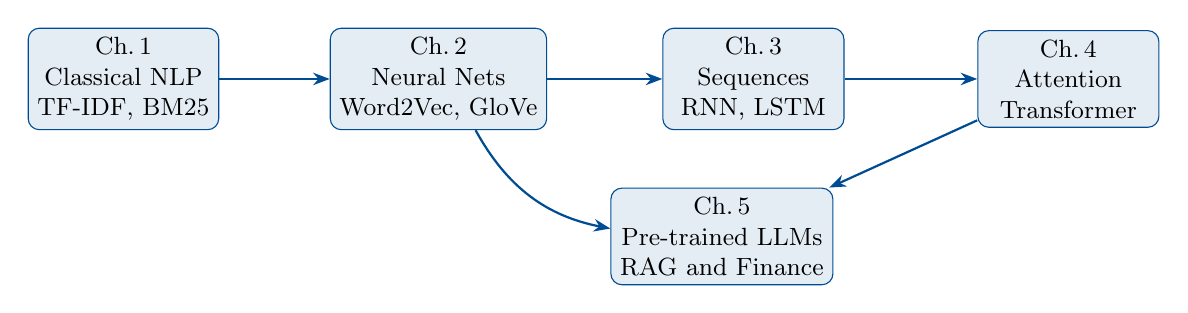
\begin{tikzpicture}[
    box/.style={draw=uniblue, fill=uniblue!10, rounded corners=4pt,
                minimum width=2.3cm, minimum height=1.1cm,
                align=center, font=\small},
    arr/.style={-{Stealth[length=6pt]}, thick, uniblue}
  ]
    \node[box](c1) at (-2, 0)    {Ch.\,1\\Classical NLP\\TF-IDF, BM25};
    \node[box](c2) at (2 ,0)   {Ch.\,2\\Neural Nets\\Word2Vec, GloVe};
    \node[box](c3) at (6,0)   {Ch.\,3\\Sequences\\RNN, LSTM};
    \node[box](c4) at (10,0)   {Ch.\,4\\Attention\\Transformer};
    \node[box](c5) at (5.6,-2.0){Ch.\,5\\Pre-trained LLMs\\RAG and Finance};
    \draw[arr](c1)--(c2); \draw[arr](c2)--(c3);
    \draw[arr](c3)--(c4); \draw[arr](c4)--(c5);
    \draw[arr](c2) to[bend right=25] (c5);
  \end{tikzpicture}
  \end{center}
  \vspace{0.3em}
  \begin{block}{The guiding question of Chapter~1 -- finally answered}
    \emph{How does a language system represent, compare, retrieve,
    and generate text?}\\[0.3em]
    \textbf{Represent:} Ch.\,1--4 (sparse $\to$ dense $\to$ contextual).\\
    \textbf{Compare:} Ch.\,1 (BM25, cosine), Ch.\,5 (bi-encoder).\\
    \textbf{Retrieve:} Ch.\,5 (FAISS, hybrid, RAG).\\
    \textbf{Generate:} Ch.\,4--5 (transformer decoder, GPT, LLMs).
  \end{block}
\end{frame}
%
%..................................................................
%
\begin{frame}{References}
  \begin{itemize}
    \setlength\itemsep{0.2em}
    \small
    \item Devlin et al.\ (2019). BERT. \textit{NAACL-HLT}.
    \item Liu et al.\ (2019). RoBERTa. \textit{arXiv:1907.11692}.
    \item Yang et al.\ (2020). FinBERT. \textit{IJCAI}.
    \item Reimers \& Gurevych (2019). Sentence-BERT. \textit{EMNLP}.
    \item Brown et al.\ (2020). GPT-3. \textit{NeurIPS}.
    \item Ouyang et al.\ (2022). InstructGPT / RLHF. \textit{NeurIPS}.
    \item Hoffmann et al.\ (2022). Chinchilla. \textit{NeurIPS}.
    \item Rafailov et al.\ (2023). DPO. \textit{NeurIPS}.
    \item Wei et al.\ (2022). Emergent Abilities. \textit{TMLR}.
    \item Schaeffer et al.\ (2023). Are Emergent Abilities a Mirage? \textit{NeurIPS}.
    \item Lewis et al.\ (2020). RAG. \textit{NeurIPS}.
    \item Johnson et al.\ (2019). FAISS. \textit{IEEE Trans.\ Big Data}.
    \item Shahul et al.\ (2023). RAGAS. \textit{arXiv:2309.15217}.
    \item Sanh et al.\ (2020). DistilBERT. \textit{EMC\textsuperscript{2} NeurIPS Workshop}.
  \end{itemize}
\end{frame}
%
%===================================================================================================
%
\end{document}
%
%===================================================================================================
%


%
%..................................................................
%
\begin{frame}{The Pre-training / Fine-tuning Pipeline}
  \begin{center}
  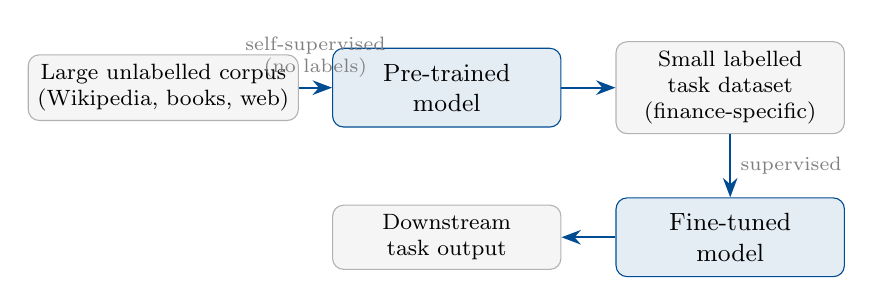
\begin{tikzpicture}[
    box/.style={draw=uniblue, fill=uniblue!10, rounded corners=4pt,
                minimum width=2.9cm, minimum height=1.0cm,
                align=center, font=\small},
    dat/.style={draw=gray!60, fill=gray!8, rounded corners=4pt,
                minimum width=2.9cm, minimum height=0.75cm,
                align=center, font=\footnotesize},
    arr/.style={-{Stealth[length=7pt]}, thick, uniblue},
    lab/.style={font=\scriptsize, gray, align=center}
  ]
    \node[dat] (corp)  at (0,  0)  {Large unlabelled corpus\\(Wikipedia, books, web)};
    \node[box] (pre)   at (3.6, 0) {Pre-trained\\model};
    \node[dat] (task)  at (7.2, 0) {Small labelled\\task dataset\\(finance-specific)};
    \node[box] (ft)    at (7.2,-1.9){Fine-tuned\\model};
    \node[dat] (out)   at (3.6,-1.9){Downstream\\task output};

    \draw[arr](corp)--node[above,lab]{self-supervised\\(no labels)}(pre);
    \draw[arr](pre)--(task);
    \draw[arr](task)--node[right,lab]{supervised}(ft);
    \draw[arr](ft)--(out);
  \end{tikzpicture}
  \end{center}
  \begin{alertblock}{Why this matters for finance}
    Labelled financial data is scarce and expensive.
    Pre-training allows the model to absorb language knowledge from large
    general corpora; a small domain-specific labelled set suffices for
    fine-tuning.
  \end{alertblock}
\end{frame}
%
%..................................................................
%
\begin{frame}{Sentence-BERT: From Token Vectors to Sentence Vectors}
  \textbf{Problem:} BERT produces one vector per token.
  For semantic search and sentence similarity, we need a
  \emph{single fixed-size} sentence vector.

  Using the raw \texttt{[CLS]} vector gives poor results on
  semantic similarity benchmarks.  Naive mean-pooling is only
  marginally better.

  \medskip
  \textbf{Sentence-BERT} (Reimers \& Gurevych, 2019):
  fine-tune a siamese BERT with a contrastive or regression objective
  on sentence pairs.  After training:
  \[
    \mathbf{s} \;=\; \frac{1}{n}\sum_{i=1}^{n}\mathbf{h}_i
    \;\in\;\mathbb{R}^{768}
  \]
  is a high-quality sentence embedding suitable for cosine similarity.

  \begin{block}{Forward reference to Part~V (RAG)}
    Sentence-BERT is the canonical \emph{bi-encoder} used for dense
    retrieval.  This is the direct connection to the promise from
    Chapter~1: \emph{``Lesson~4 will show how these vectors drive
    retrieval and RAG.''}
  \end{block}
\end{frame}
